\def\CTeXPreproc{Created by ctex v0.2.9, don't edit!}
%\documentclass{beamer}
\documentclass[%handout,
xcolor=pdftex]{beamer}
\mode<presentation> {
  \usetheme{Warsaw}
  \setbeamercovered{transparent}
}
\let\Tiny=\tiny
\usetheme{Singapore}
\usecolortheme{dolphin}
\usepackage{amsmath}
\usepackage{textcomp}
\usepackage{amssymb}
\usepackage{amsthm}
\usepackage{graphicx}
\usepackage{color}
\usepackage{lipsum}
\usepackage{hyperref}
\usepackage{multirow}
\usepackage{bm}
%\setbeamertemplate{headline}{}
\setbeamertemplate{footline}[page number]
\newcommand\Fontvi{\fontsize{9pt}{8}\selectfont}
\newcommand\Fontvii{\fontsize{7pt}{8}\selectfont}
\newcommand{\backupbegin}{
   \newcounter{finalframe}
   \setcounter{finalframe}{\value{framenumber}}
}
\newcommand{\backupend}{
   \setcounter{framenumber}{\value{finalframe}}
}\newtheorem{proposition}{Proposition}
\title{Unit 4: Review of Regression}
\author[STAT 5170: Applied Time Series, Unit 4]{Taylor R. Brown PhD}
\institute{Department of Statistics, University of Virginia}
\date{Spring 2020}

\AtBeginSubsection[] {
  \begin{frame}<beamer>{Outline}
    \tableofcontents[currentsection,currentsubsection]
  \end{frame}
}

\begin{document}


\frame{\titlepage}


\begin{frame}
\frametitle{Readings for Unit 4}

Textbook chapter 2.1.

\end{frame}

\begin{frame}
\frametitle{Last Unit}
\begin{enumerate}
\item Stationarity
\item Autocovariance and Autocorrelation of Stationary Time Series
\item Estimating the ACF
\end{enumerate}\end{frame}

\begin{frame}
\frametitle{This Unit}
\begin{enumerate}
\item Parameter Estimation
\item Model Selection
\item Diagnostics
\end{enumerate}
\end{frame}

\begin{frame}
\frametitle{Motivation}
In time series analysis, we frequently would prefer to analyze a stationary process.  This allows us to better estimate autocorrelation and other quantities of interest.  In addition,  ARMA processes provide a rich framework for analyzing stationary processes. A strong trend, however, may \textbf{obscure} the behavior of the stationary process. It may, therefore, be necessary to \textbf{remove} a trend; one way to do that is via regression.

\end{frame}

\section{Linear Regression Basics}
\frame{\tableofcontents[currentsection]}

\begin{frame}
\frametitle{Linear Regression Basics}

The basic data type for regression consists of a list of pairs of numbers, $(x_1,z_1),..., (x_n, z_n)$, where the $x_i$ are thought of as the response variables and $z_i$ are thought of as the predictor variables.  The simple linear regression model would then be
$$
x_t= \beta_0 + \beta_1 z_t + w_t
$$
for $t=1,..,n$ where $w_t, t=1,...,n$ are zero-mean iid normal random variables with variance $\sigma_w^2$.


\end{frame}



\begin{frame}
\frametitle{Linear Regression Basics}

We can extend this to multiple predictors with a model

\begin{equation*}
x_t= \beta_0 + \beta_1 z_{t1} +...+  \beta_q z_{tq} + w_t.
\end{equation*}

Using vector notation, the linear regression model can be written as

\begin{equation} \label{eq:full}
x_t=  \boldsymbol{\beta^{\prime}z_t} + w_t
\end{equation}

where $\boldsymbol{\beta^{\prime}} = (\beta_0,\beta_1,\cdots,\beta_q)$ and $\boldsymbol{z_t}=(1,z_{t1},z_{t2},\cdots,z_{tq})^{\prime}$.

\end{frame}

\section{Parameter Estimation}
\frame{\tableofcontents[currentsection]}

\begin{frame}
\frametitle{Parameter Estimation}

Estimating the parameter vector $\boldsymbol{\beta}$ is done by minimizing the error sum of squares

\begin{equation}
Q = \sum_{t=1}^{n}  ( x_t - \boldsymbol{\beta^{\prime}z_t})^2
\end{equation}

with respect to $\beta_0, \beta_1, \cdots, \beta_q$. Let the matrix $\boldsymbol{Z} = (1, z_{1},z_{2},\cdots,z_{n})^{\prime}$ be the $n \times (q+1)$ matrix of $n$ samples of the predictor variables, and $\boldsymbol{x} = (x_{1},x_{2},\cdots,x_{n})^{\prime}$ the vector of response variables. It turns out that

\begin{equation}
\boldsymbol{\hat{\beta}} = \boldsymbol{(Z^{\prime}Z)^{-1}Z^{\prime}x}
\end{equation}

The estimators $\boldsymbol{\hat{\beta}}$ are unbiased, and are called \textbf{ordinary least squares estimators}.

\end{frame}

\begin{frame}
\frametitle{Parameter Estimation}

The minimized error sum of squares, denoted by $SSE$, is

\begin{equation}
SSE = \sum_{t=1}^{n}  ( x_t - \boldsymbol{\hat{\beta}^{\prime}z_t})^2
\end{equation}

\end{frame}

\begin{frame}
\frametitle{Parameter Estimation}

An unbiased estimator for the variance $\sigma_w^2$ is

\begin{equation}
s_w^2 = MSE = \frac{SSE}{n-(q+1)}.
\end{equation}

\end{frame}

\begin{frame}
\frametitle{Other Terminology}

\textbf{Fitted values}:

\begin{equation}
\hat{x_t} = \hat{\boldsymbol{\beta}}^{\prime}\boldsymbol{z_t}.
\end{equation}

\textbf{Residuals}:

\begin{equation}
e_i = x_t - \hat{x_t}.
\end{equation}

\end{frame}

\begin{frame}
\frametitle{Inference}

Assuming independent Gaussian errors, we can build confidence intervals using statistics such as
$$
\frac{\hat{\beta_i} -\beta_i}{\mbox{standard error}(\hat\beta_i)}
$$
which have a t-distribution with $n-(q+1)$ d.f, and $s_w^2$ is distributed proportionally to a $\chi^2_{n-(q+1)}$.

\end{frame}

\section{Model Selection}
\frame{\tableofcontents[currentsection]}

\begin{frame}
\frametitle{Model Selection: Nested Models}

Often times, we want to compare various competing models or select a subset of predictors. Consider a model that only has a subset $r < q$ predictors $\boldsymbol{z_{t,1:r}} = (z_{t1},z_{t2},\cdots,z_{tr})^{\prime}$,

\begin{equation} \label{eq:reduced}
x_t = \boldsymbol{\beta_r^{\prime}z_{t,1:r}} + w_t.
\end{equation}

(\ref{eq:reduced}) is called the \textbf{reduced} model, and is compared with the \textbf{full} model, as specified in (\ref{eq:full}), which has all $q$ predictor variables. Models (\ref{eq:full}) and (\ref{eq:reduced}) are called \textbf{nested} models since all the terms in the reduced model occur in the full model.

\end{frame}

\begin{frame}
\frametitle{Model Selection: Nested Models}

With nested models, we compare the $SSE$ of both models using the partial $F$ statistic

\begin{equation}
F_{q-r,n-q-1} = \frac{SSE_r - SSE}{SSE} \frac{n-q-1}{q-r},
\end{equation}

where $SSE_r$ denotes the $SSE$ of the reduced model.

\end{frame}

\begin{frame}
\frametitle{Model Selection: Non-Nested Models}

When comparing non-nested models, we can use the Akaike's Information Criterion (AIC)

\begin{equation}
\mbox{AIC} = \log \hat{\sigma_k}^2+\frac{n+2k}{n},
\end{equation}

where $\hat{\sigma_k}^2 = \frac{SSE(k)}{n}$ and $SSE(k)$ is the $SSE$ for a model with $k$ regression coefficients. For model selection, we would like to \textbf{minimize} the AIC.

\end{frame}

\begin{frame}
\frametitle{Coefficient of Determination}

The coefficient of determination, $R^2$, is a popular measure of model fit. For example, for the full model,

\begin{equation}
R^2 = \frac{SSE_0 - SSE}{SSE_0},
\end{equation}

where $SSE_0$ is the total sum of squares. $R^2$ is interpreted as the proportion of the variance in the response variable that can be explained by our model. \\

\vspace{5mm}

\textbf{Question:} When should $R^2$ be used / not used?

\end{frame}

\section{Diagnostics}
\frame{\tableofcontents[currentsection]}

\begin{frame}
\frametitle{Assumptions for Linear Regression}

The assumptions for linear regression are

\begin{itemize}
\item There exist a linear relationship between the response and predictor variables.
\item $\mbox{E}(w_i) = 0$.
\item $\mbox{Var}(w_i) = \sigma_w^2$ is constant and finite.
\item $w_i$'s are uncorrelated.
\item $w_i$ are iid normal.
\end{itemize}

\end{frame}

\begin{frame}
\frametitle{Diagnostics}

Use the following to check regression assumptions are satisfied:

\begin{itemize}
\item Residual plot: to check if right regression equation used, variance of errors is constant, mean of errors is zero.
\item ACF plot: to determine correlation.
\item Normal probability plot: to check for normality.
\end{itemize}

\end{frame}

\section{Worked Example}
\frame{\tableofcontents[currentsection]}

\begin{frame}
\frametitle{Marriages in Church of England}

In this example, we go back to the data regarding number of marriages in the Church of England.

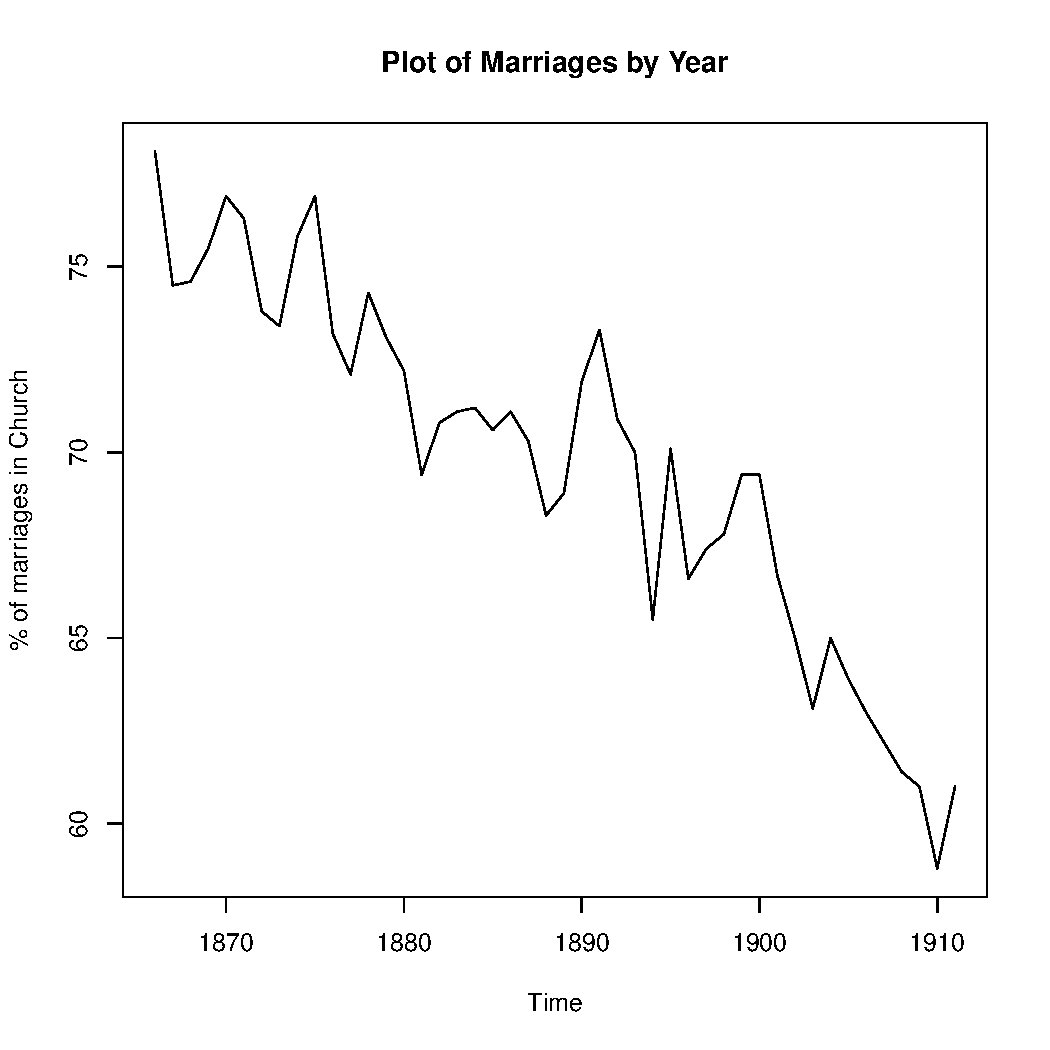
\includegraphics[width=100mm, height=50mm]{pics/marriagesplot.pdf}

We choose to fit a simple linear regression because of the apparent decreasing trend.

\end{frame}

\begin{frame}[fragile]
\frametitle{Marriages in Church of England}

\begin{verbatim}
> timefit<-lm(marriages~time)
> summary(timefit)

Coefficients:
             Estimate Std. Error t value Pr(>|t|)
(Intercept) 704.78168   37.93471   18.58   <2e-16 ***
time         -0.33629    0.02009  -16.74   <2e-16 ***

Residual standard error: 1.809 on 44 degrees of freedom
Multiple R-squared: 0.8643,     Adjusted R-squared: 0.8612
F-statistic: 280.3 on 1 and 44 DF,  p-value: < 2.2e-16

> AIC(timefit)
[1] 189.0146
\end{verbatim}

\end{frame}

\begin{frame}
\frametitle{Marriages in Church of England}

Check residual plot.

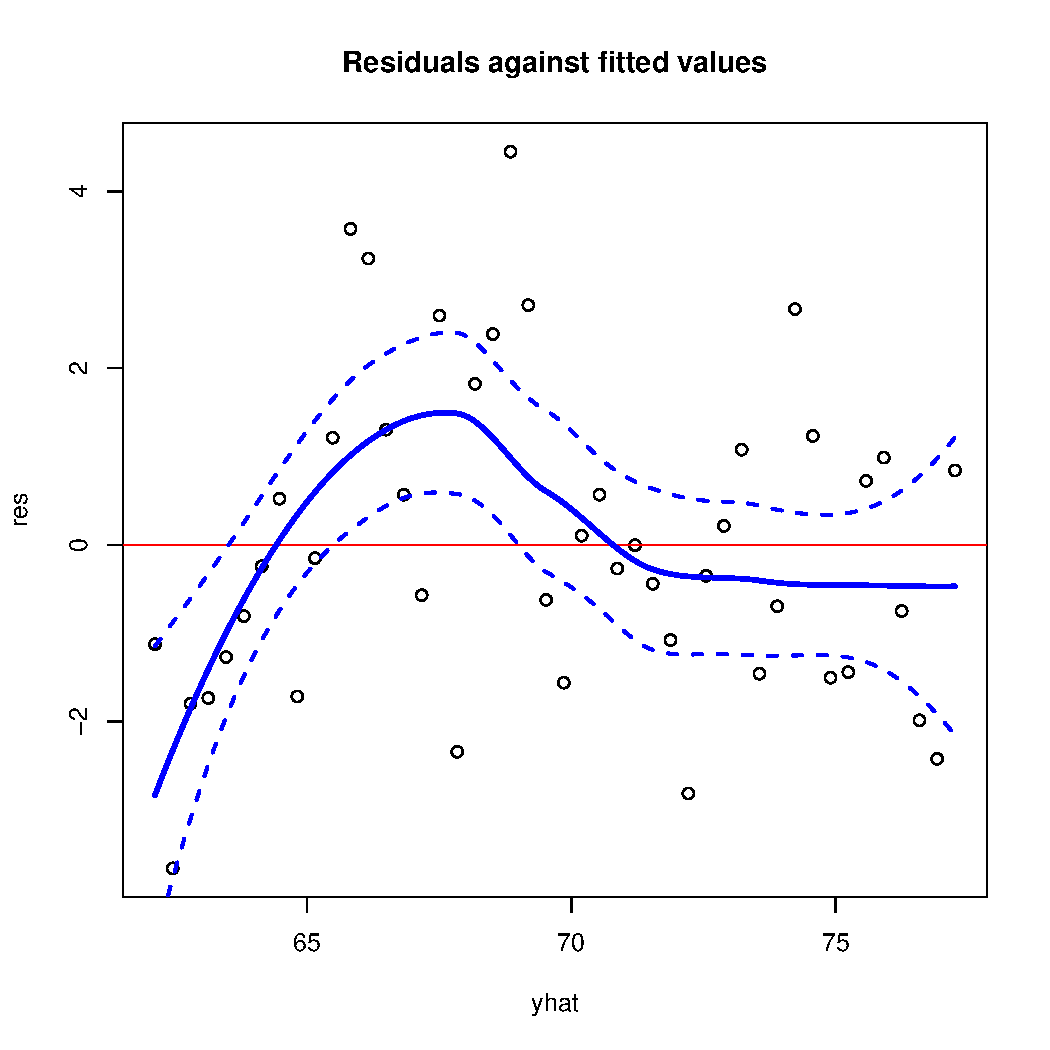
\includegraphics[width=100mm, height=60mm]{pics/residtimefit.pdf}

Curvature present. Let's add a square term for time.

\end{frame}

\begin{frame}[fragile]
\frametitle{Marriages in Church of England}

\begin{verbatim}
> timesq<-time^2
> timefitsq<-lm(marriages~time+timesq)
> anova(timefitsq)
Analysis of Variance Table

Response: marriages
          Df Sum Sq Mean Sq  F value    Pr(>F)
time       1 916.90  916.90 324.6874 < 2.2e-16 ***
timesq     1  22.50   22.50   7.9682  0.007182 **
Residuals 43 121.43    2.82

> AIC(timefitsq)
[1] 183.1945
\end{verbatim}

P-value for timesq is significant. AIC has gone down, indicating the fit of the model has improved.

\end{frame}

\begin{frame}
\frametitle{Marriages in Church of England}

Check residual plot.

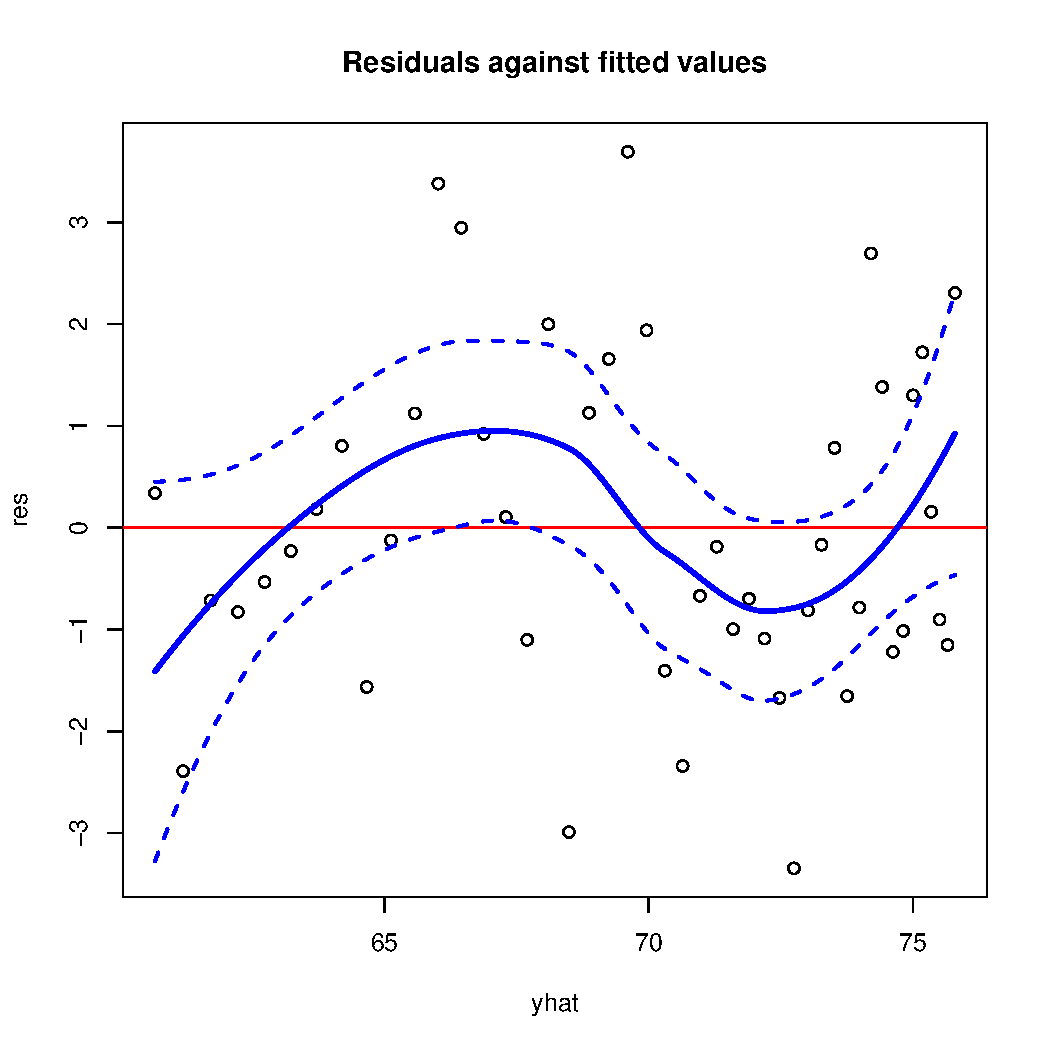
\includegraphics[width=100mm, height=60mm]{pics/residtimefitsq.pdf}

\end{frame}

\begin{frame}
\frametitle{Marriages in Church of England}

Check ACF plot.

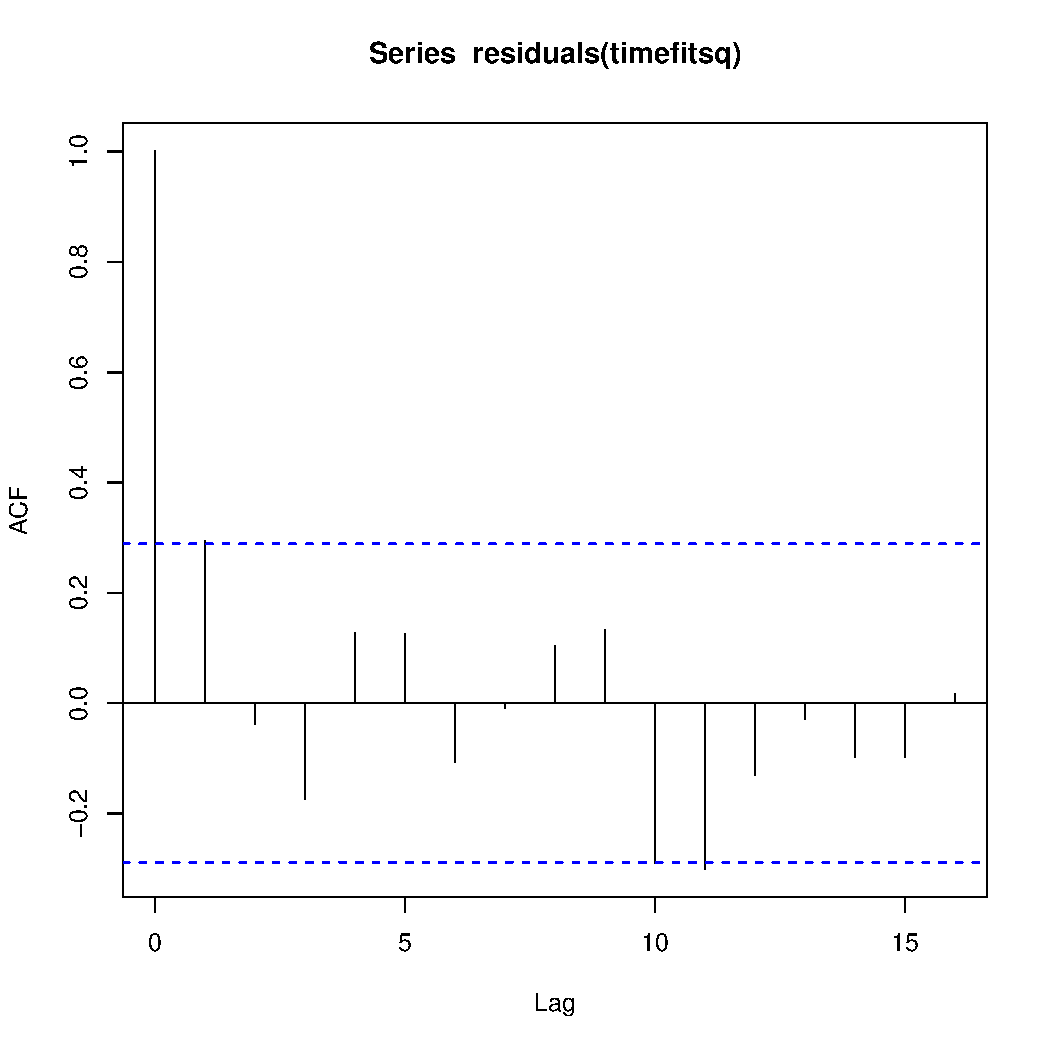
\includegraphics[width=100mm, height=60mm]{pics/acftimefitsq.pdf}

\end{frame}

\begin{frame}
\frametitle{Marriages in Church of England}

Check QQ plot.

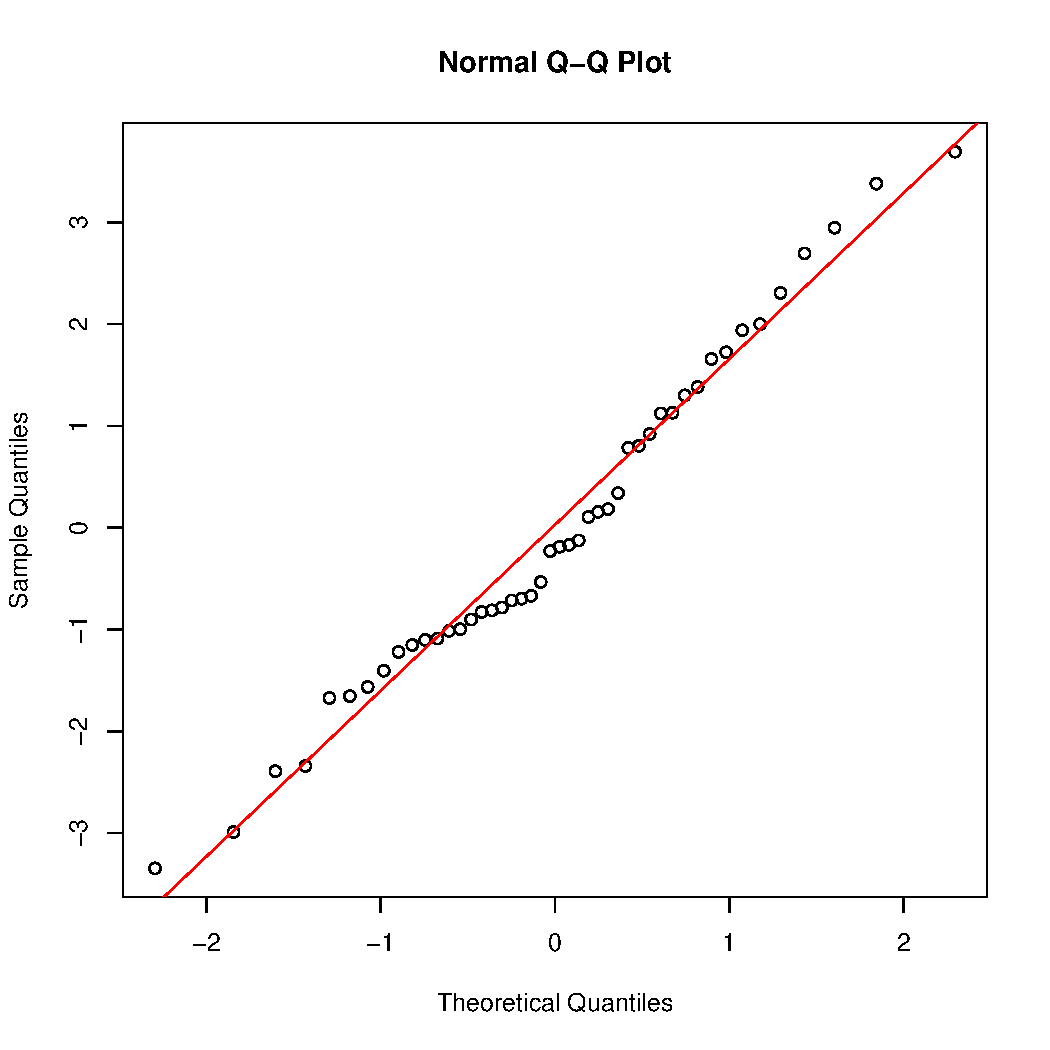
\includegraphics[width=100mm, height=60mm]{pics/qqnormtimefitsq.pdf}

\end{frame}

\begin{frame}
\frametitle{Marriages in Church of England and Mortality Rate}

Another possibility is that we wish to compare two time series via regression.  We can treat one series as fixed, and the other series as simply a linearly transformed, perturbed version of that series. For example, is the percentage of marriages in the Church of England linearly related to the mortality rate in England?

\end{frame}

\begin{frame}[fragile]
\frametitle{Marriages in Church of England and Mortality Rate}

\begin{verbatim}
> comparefit<-lm(marriages~mortality)
> summary(comparefit)

Coefficients:
            Estimate Std. Error t value Pr(>|t|)
(Intercept)  30.0553     1.9439   15.46   <2e-16 ***
mortality     2.1633     0.1054   20.52   <2e-16 ***

Residual standard error: 1.51 on 44 degrees of freedom
Multiple R-squared: 0.9054,     Adjusted R-squared: 0.9033
F-statistic: 421.3 on 1 and 44 DF,  p-value: < 2.2e-16

> AIC(comparefit)
[1] 172.4094
\end{verbatim}

\end{frame}

\begin{frame}
\frametitle{Marriages in Church of England and Mortality Rate}

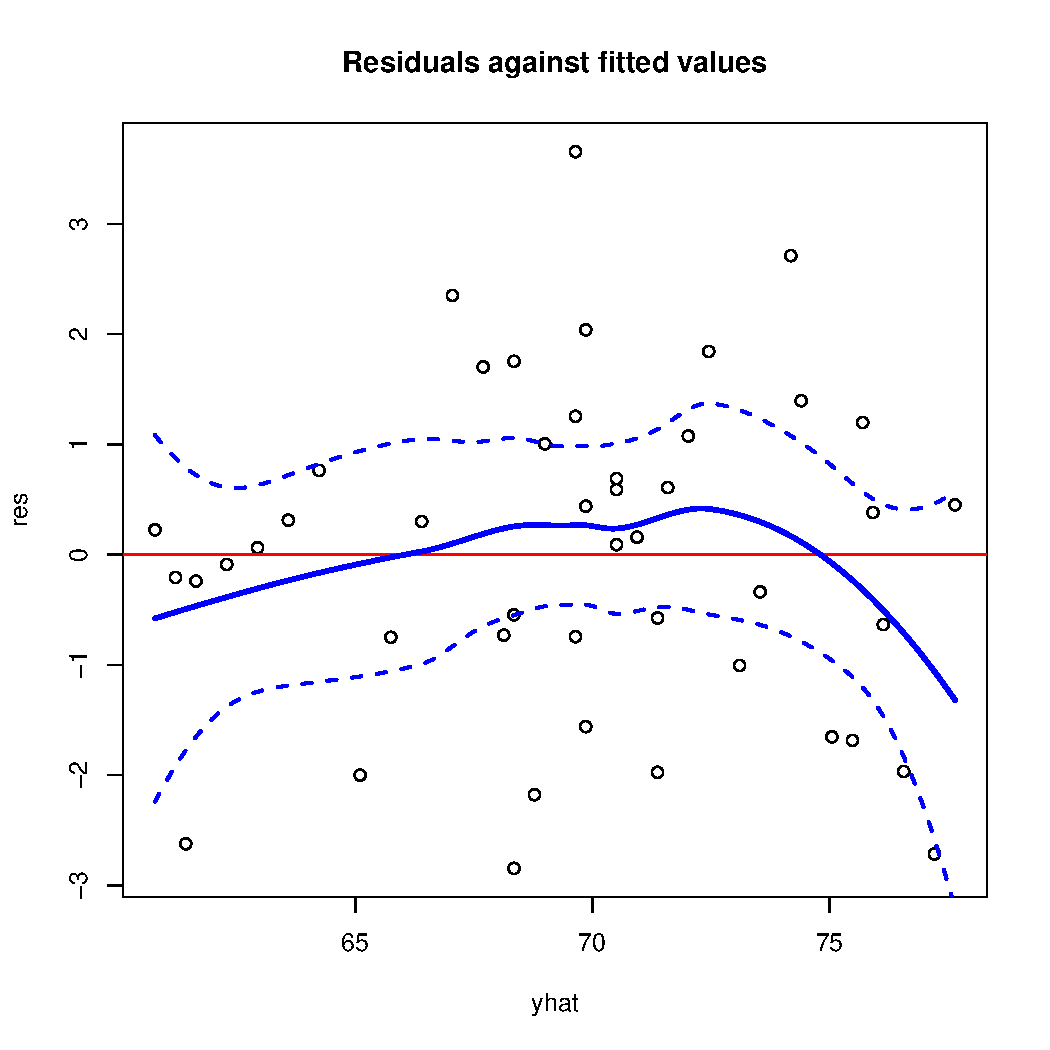
\includegraphics[width=100mm, height=60mm]{pics/residcomparefit.pdf}

\end{frame}

\begin{frame}
\frametitle{Marriages in Church of England and Mortality Rate}


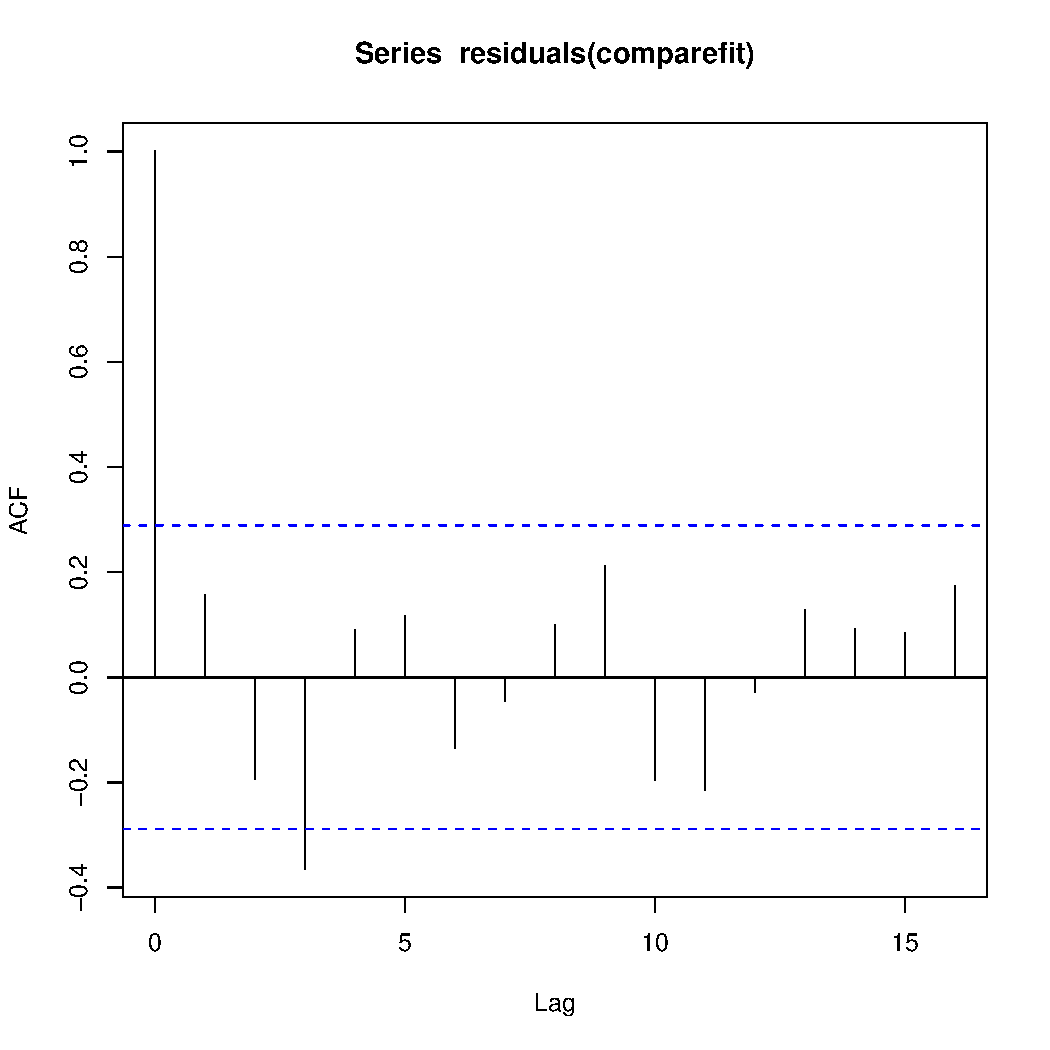
\includegraphics[width=100mm, height=60mm]{pics/acfcomparefit.pdf}

\end{frame}

\begin{frame}
\frametitle{Marriages in Church of England and Mortality Rate}

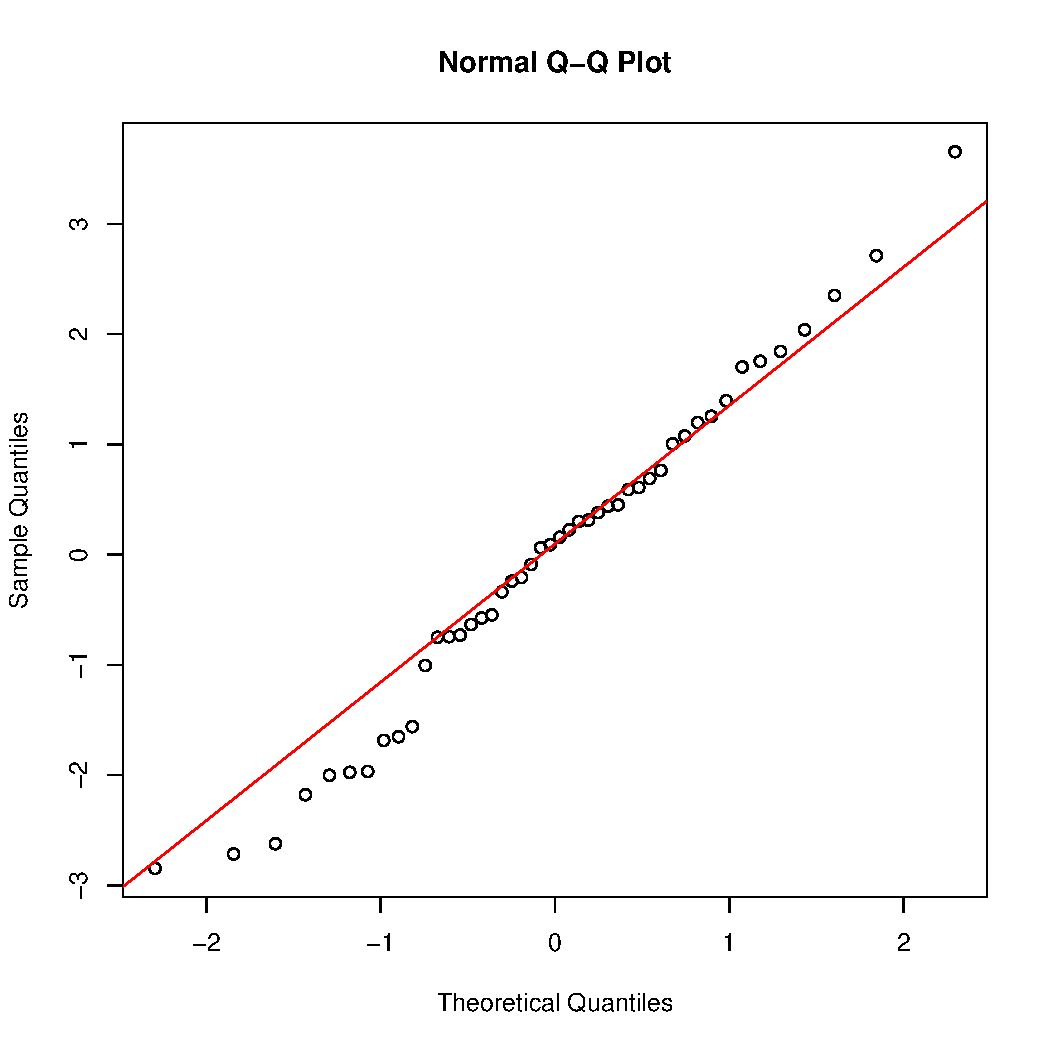
\includegraphics[width=100mm, height=60mm]{pics/qqnormcomparefit.pdf}

\end{frame}

\begin{frame}[fragile]
\frametitle{Marriages in Church of England against Mortality Rate and Year}

Use both mortality rate and year as predictor variables.

\begin{verbatim}
> comparetimefit<-lm(marriages~mortality+time)
> anova(comparetimefit)
Analysis of Variance Table

Response: marriages
          Df Sum Sq Mean Sq F value Pr(>F)
mortality  1 960.52  960.52 416.149 <2e-16 ***
time       1   1.07    1.07   0.464 0.4994
Residuals 43  99.25    2.31

> AIC(comparetimefit)
[1] 173.9157
\end{verbatim}

\end{frame}


\end{document} 